%% V1.0
%% by Gabriel Garcia, gabrcg@gmail.com
%% This is a template for Udacity projects using IEEEtran.cls

%% Be Udacious!

\documentclass[10pt,journal,compsoc]{IEEEtran}

\usepackage[pdftex]{graphicx}
\usepackage{cite}
\hyphenation{op-tical net-works semi-conduc-tor}


\begin{document}

\title{Udacity RoboND Project: Robotic Inference \\
    \huge Image Classification Using GoogLeNet}

\author{Trijeet Kr. Modak}

\markboth{Inference project, Robotic Nanodegree, Udacity}%
{}
\IEEEtitleabstractindextext{%

\begin{abstract}
This paper explores a deep neural network architecture, GoogLeNet, to classify objects on a conveyor belt or lying on any flat surface. Training, validation and testing of the model is performed over Nvidia DIGITS platform which simplifies the data and model management process. Data acquisition, training and results are also discussed in this paper. The final accuracy of the models and the inference time met the project requirements.
\end{abstract}

% Note that keywords are not normally used for peerreview papers.
\begin{IEEEkeywords}
Robot, GoogLeNet, Udacity, neural network, deep learning, classification.
\end{IEEEkeywords}}


\maketitle
\IEEEdisplaynontitleabstractindextext
\IEEEpeerreviewmaketitle
\section{Introduction}
\label{sec:introduction}

\IEEEPARstart{I}{t} is important for robots to understand its surroundings correctly to carry out the operation(s) it has been assigned with. One of the simplest yet elegant way to achieve this is through vision, i.e. using cameras attached to a robot and processing the video feeds from them. Such processing includes techniques such as image classification, object detection in images, motion detection, etc. This paper focuses on image classification using which the a robot can identify and classify known objects in its surrounding.

Pattern recognition and machine learning \cite{nasrabadi2007pattern} algorithms such as Deep Neural Networks \cite{schmidhuber2015deep} can simplify the task of object classification by learning the features of the objects. A neural network can be trained with existing labeled images of various objects and later can be used to identify the objects from a previously unseen image. Hence, if a robot is equipped with such a trained model, it can quickly infer the objects in its surrounding from its camera feeds. GoogLeNet \cite{szegedy2015going} is one such architecture that won the ImageNet \cite{deng2009imagenet} 2014 challenge. Hence GoogLeNet is used for classification of the images in this project as it is faster and has a high accuracy rate.

\section{Background / Formulation}

DIGITS \cite{yeager2015digits} is a deep learning platform by NVIDIA that simplifies the entire model training process. It provides a few pre-trained models such as LeNet, AlexLet and GoogLeNet. It also allows custom models to be imported and used. It also handles creation and management of datasets for the model training. As a result, DIGITS was chosen to train the models. 

There are two parts to the project where two models are to be trained, each to classify and detect items as listed below:

\begin{itemize}
\item Classes for Object Detection on Conveyor Belt (Model 1 - Udacity Dataset):
\end {itemize}

\begin{enumerate}
\setlength{\itemindent}{+.2in}
\item Bottle, 
\item Candy Box, and
\item Nothing
\end{enumerate}

\begin{itemize}
\item Classes for Object Detection on self collected data (Model 2 - Collected Dataset):
\end {itemize}

%example for numbered list
\begin{enumerate}
\setlength{\itemindent}{+.2in}
\item Battery, 
\item Breadboard,
\item DC Motor, and
\item Nothing
\end{enumerate}

\section{Data Acquisition}
% \begin{figure}[thpb]
%       \centering
%       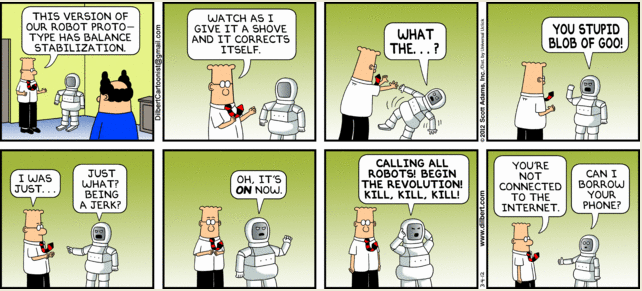
\includegraphics[width=\linewidth]{RobotRevolution5}
%       \caption{Robot Revolution.}
%       \label{fig:robot1}
% \end{figure}

\subsection{Model 1 (Udacity Dataset)}
Dataset for object detection on a conveyor belt is provided by Udacity. The following table describes the details of the dataset. The train-eval-test ratio used is 14:5:1


\begin{table}[h]
\renewcommand{\arraystretch}{1.5}
\begin{tabular}{|l|r|r|r|r|}
\hline
\textbf{Images}         & \multicolumn{1}{l|}{\textit{Bottle Images}} & \multicolumn{1}{l|}{\textit{Candy Box Images}} & \multicolumn{1}{l|}{\textit{Nothing Images}} & \multicolumn{1}{l|}{\textit{\textbf{Total}}} \\ \hline
\textit{Training}       & 3198                                        & 1747                                           & 2122                                         & 7067                                         \\ \hline
\textit{Validation}     & 1142                                        & 624                                            & 758                                          & 2524                                         \\ \hline
\textit{Testing}        & 228                                         & 124                                            & 151                                          & 503                                          \\ \hline
\textit{\textbf{Total}} & 4568                                        & 2495                                           & 3031                                         & 10094                                        \\ \hline
\end{tabular} \renewcommand{\arraystretch}{1.5} \caption{Dataset provided by Udacity}
\label{Table}
\end{table}

The following table shows a few sample images from the dataset:

\begin{table}[h]
\centering
\begin{tabular}{ccc}
Bottle & Cndy Box & Nothing \\
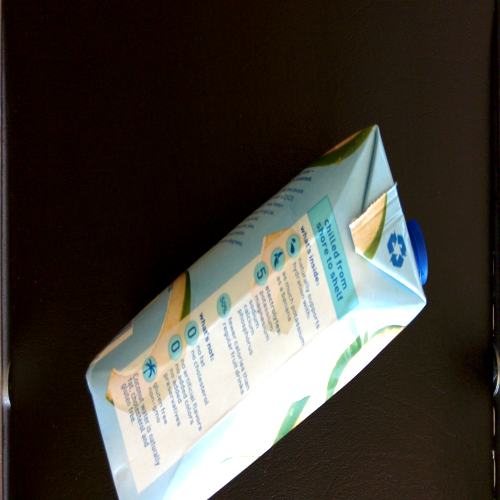
\includegraphics[scale=0.1]{imgs/coconut_1143.png} & 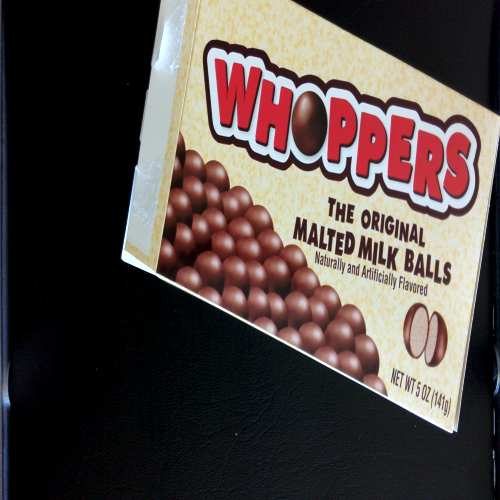
\includegraphics[scale=0.1]{imgs/woppers_972.png} & 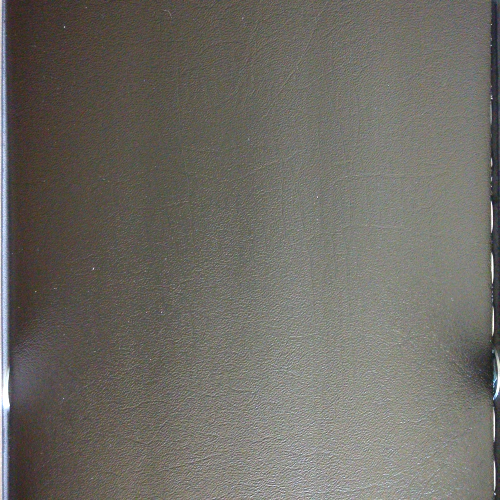
\includegraphics[scale=0.1]{imgs/Nothing_pic_103.png} \\
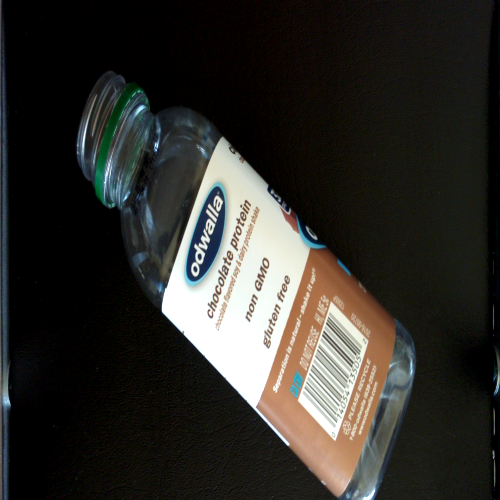
\includegraphics[scale=0.1]{imgs/odwalla_1395.png} & 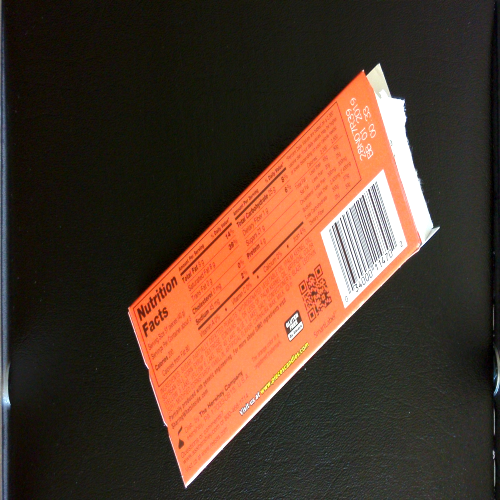
\includegraphics[scale=0.1]{imgs/reeses_685.png}   & 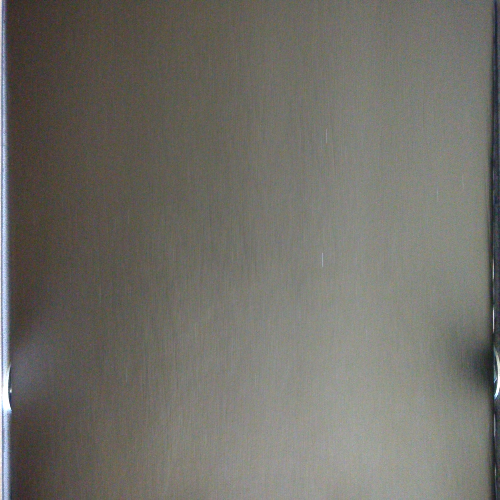
\includegraphics[scale=0.1]{imgs/Nothing_pic_1175.png}
\end{tabular}\caption{Samples from the udacity dataset}
\end{table}

\subsubsection{Model 2 (Collected Dataset)}
Images for battery, breadboard, dc motor and 'nothing' is collected placing them flat on a dark surface using Intel Realsense D435 cameras at a resolution of 640x480. The details are presented below:

\begin{table}[h]
\renewcommand{\arraystretch}{1.5}
\begin{tabular}{|l|r|r|r|l|r|}
\hline
\textit{\textbf{Images}} & \multicolumn{1}{l|}{\textit{Battery}} & \multicolumn{1}{l|}{\textit{Bread Board}} & \multicolumn{1}{l|}{\textit{DC Motor}} & \textit{Nothing} & \multicolumn{1}{l|}{\textit{\textbf{Total}}} \\ \hline
\textit{Training}        & 71                                           & 71                                               & 71                                            & 71                      & 7067                                         \\ \hline
\textit{Validation}      & 26                                           & 25                                               & 25                                            & 26                      & 2524                                         \\ \hline
\textit{Testing}         & 5                                            & 5                                                & 5                                             & 5                       & 503                                          \\ \hline
\textit{\textbf{Total}}  & 102                                          & 101                                              & 101                                           & 102                     & 406                                        \\ \hline


\end{tabular} \renewcommand{\arraystretch}{1.5} \caption{Collected Dataset}
\label{table:m2ds}
\end{table}



\begin{table}[h]
\centering
\begin{tabular}{cccc}
Battery & Bread Board & DC Motor & Nothing \\
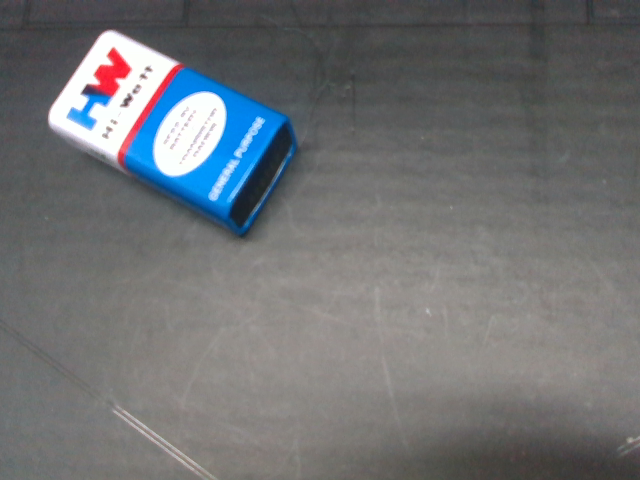
\includegraphics[scale=0.08]{imgs/battery_15.png} & 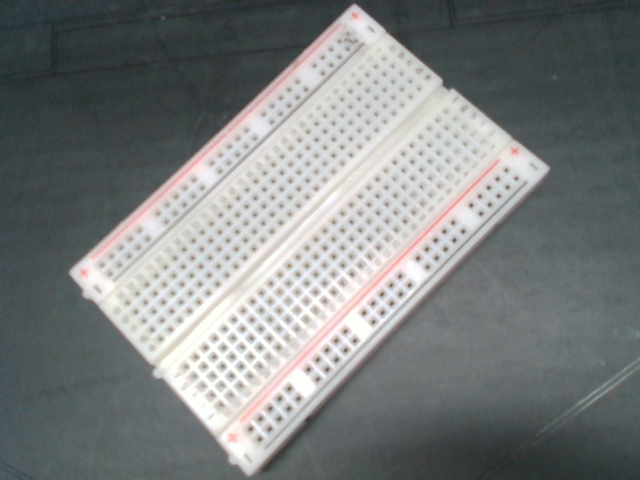
\includegraphics[scale=0.08]{imgs/bread_board_20.png} & 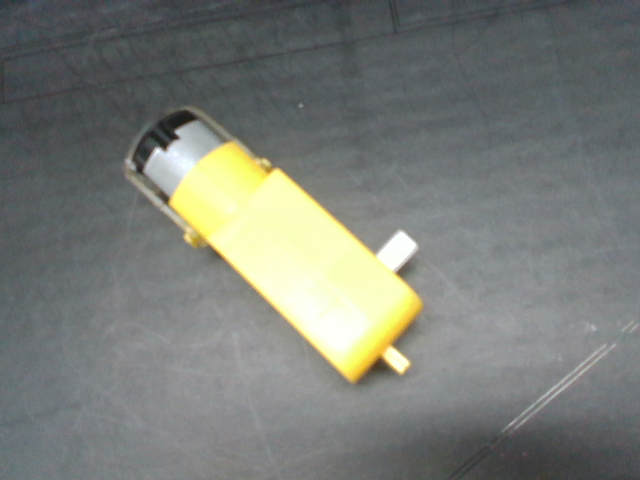
\includegraphics[scale=0.08]{imgs/dc_motor_9.png} & 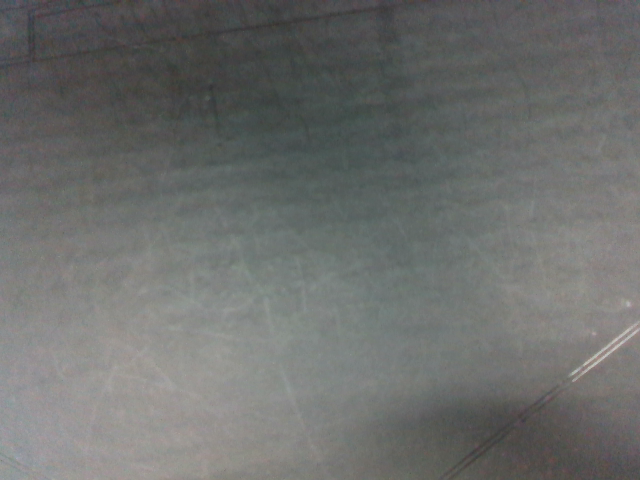
\includegraphics[scale=0.08]{imgs/nothing_7.png} \\
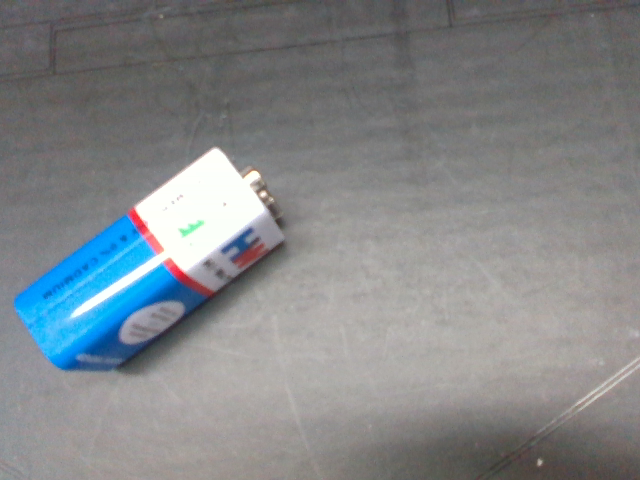
\includegraphics[scale=0.08]{imgs/battery_103.png} & 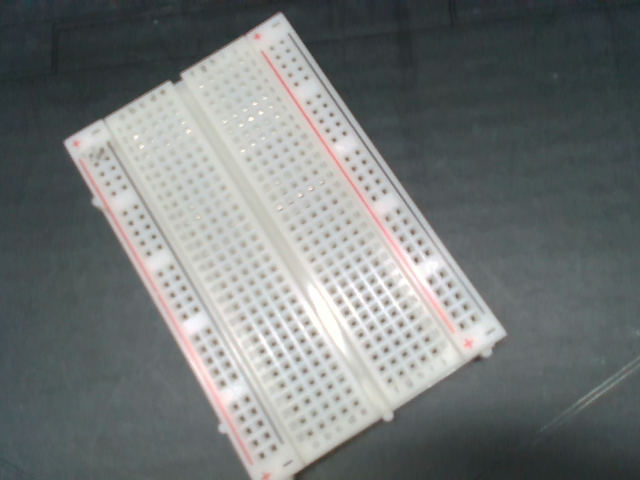
\includegraphics[scale=0.08]{imgs/bread_board_38.png}   & 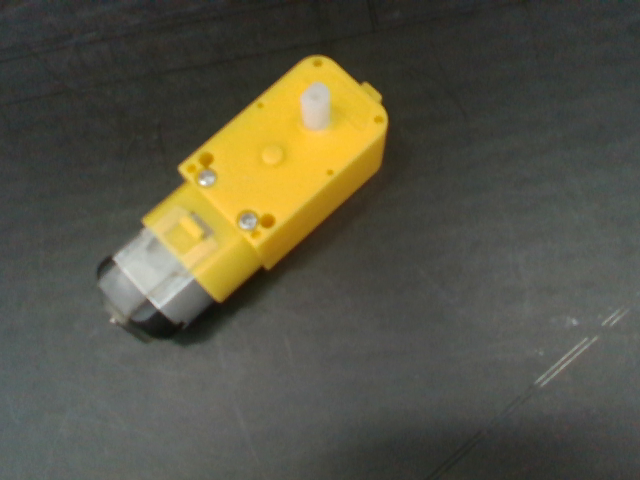
\includegraphics[scale=0.08]{imgs/dc_motor_25.png} & 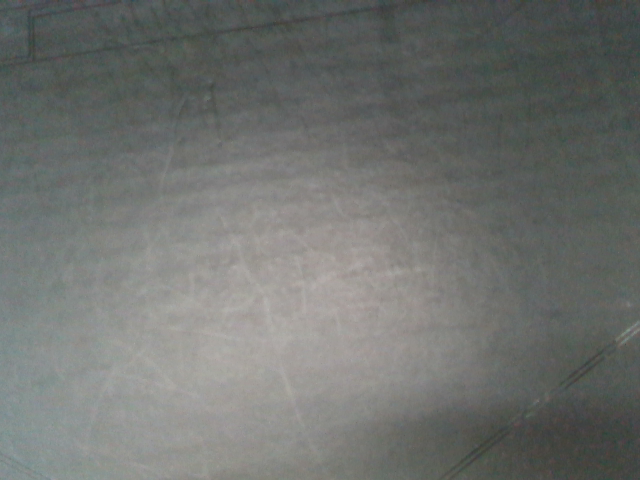
\includegraphics[scale=0.08]{imgs/nothing_96.png}
\end{tabular}\caption{Samples from the collected dataset}
\end{table}


\section{Results}
\subsection{Model 1 (Udacity Dataset)}
The model is trained for 30 epochs on the Nvidia DIGITS platform running on Tesla K80 GPU in the workspace provided by Udacity. It took slightly less than an hour to complete the training process. The training loss and accuracy curves are presented below:

\begin{figure}[h]
    \centering
    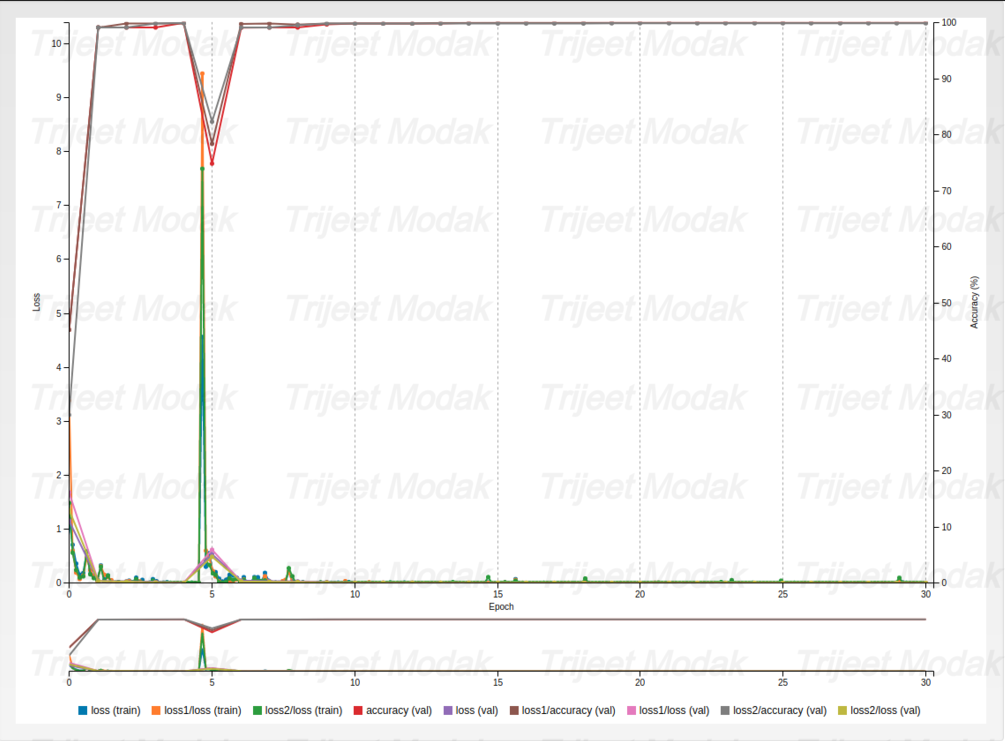
\includegraphics[scale=0.25]{imgs/loss_m1.png}
    \centering
    \caption{Model 1 loss/accuracy vs epoch curve}
    \label{fig:m1la}
\end{figure}

The result obtained on running the $evaluate$ command on the first model resulted in the output presented in the following screenshot. The model reached an accuracy of 75.40\% with an inference time of roughly 5ms which is in acceptable range of the project requirements.

\begin{figure}[h]
    \centering
    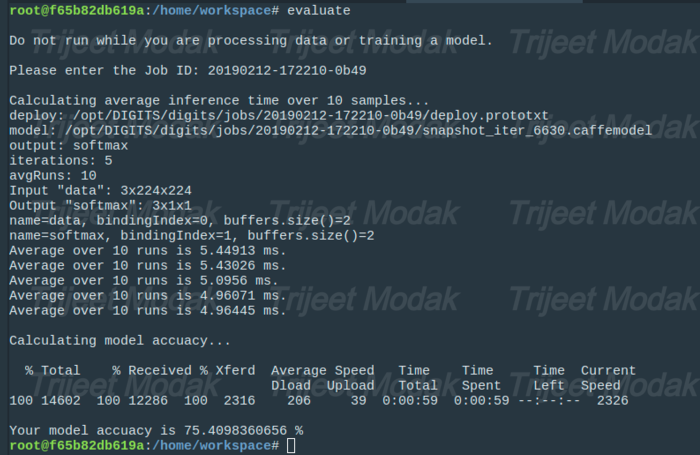
\includegraphics[scale=0.35]{imgs/evaluate.png}
    \caption{Model 1 loss/accuracy vs epoch curve}
    \label{fig:evaluate}
\end{figure}

\subsection{Model 2 (Collected Dataset)}
The second model is also trained over Nvidia DIGITS for 100 epochs which took about 10 minutes. At the end of the training it attained a validation accuracy and validation loss of 99.10\% and 0.021 respectively.
The training and validation curves are presented in the following figure:

\begin{figure}[h]
    \centering
    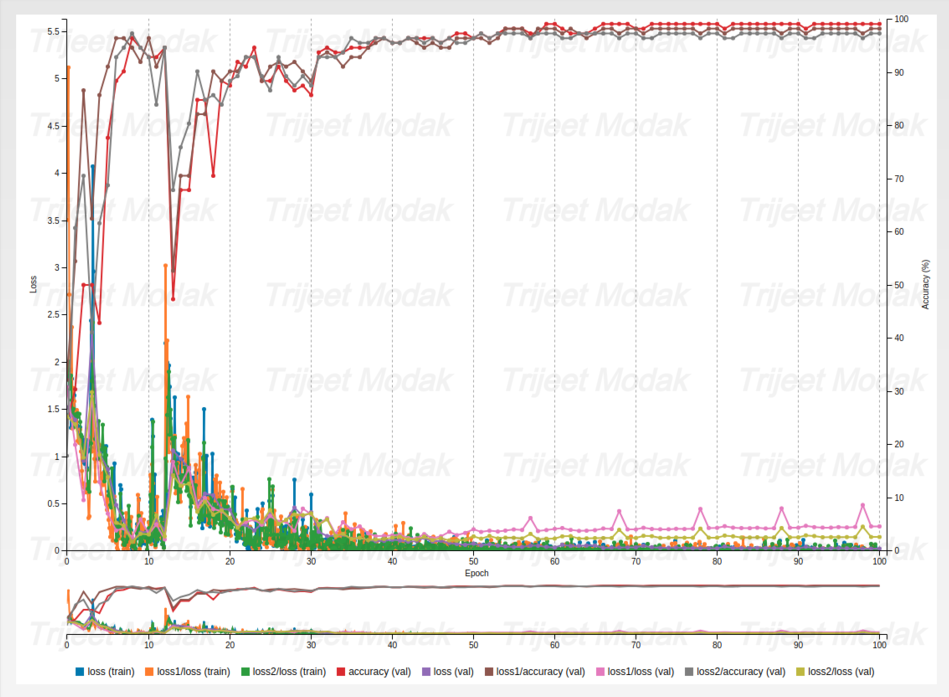
\includegraphics[scale=0.25]{imgs/loss_m2.png}
    \centering
    \caption{Model 2 loss/accuracy vs epoch curve}
    \label{fig:m1la}
\end{figure}

Once the model got trained, it is tested against a few images corresponding to the trained classes but which were not used during the training or validation process. The inference results of this model are presented in Fig. \ref{fig:detections}.

\begin{figure}[h]
    \centering
    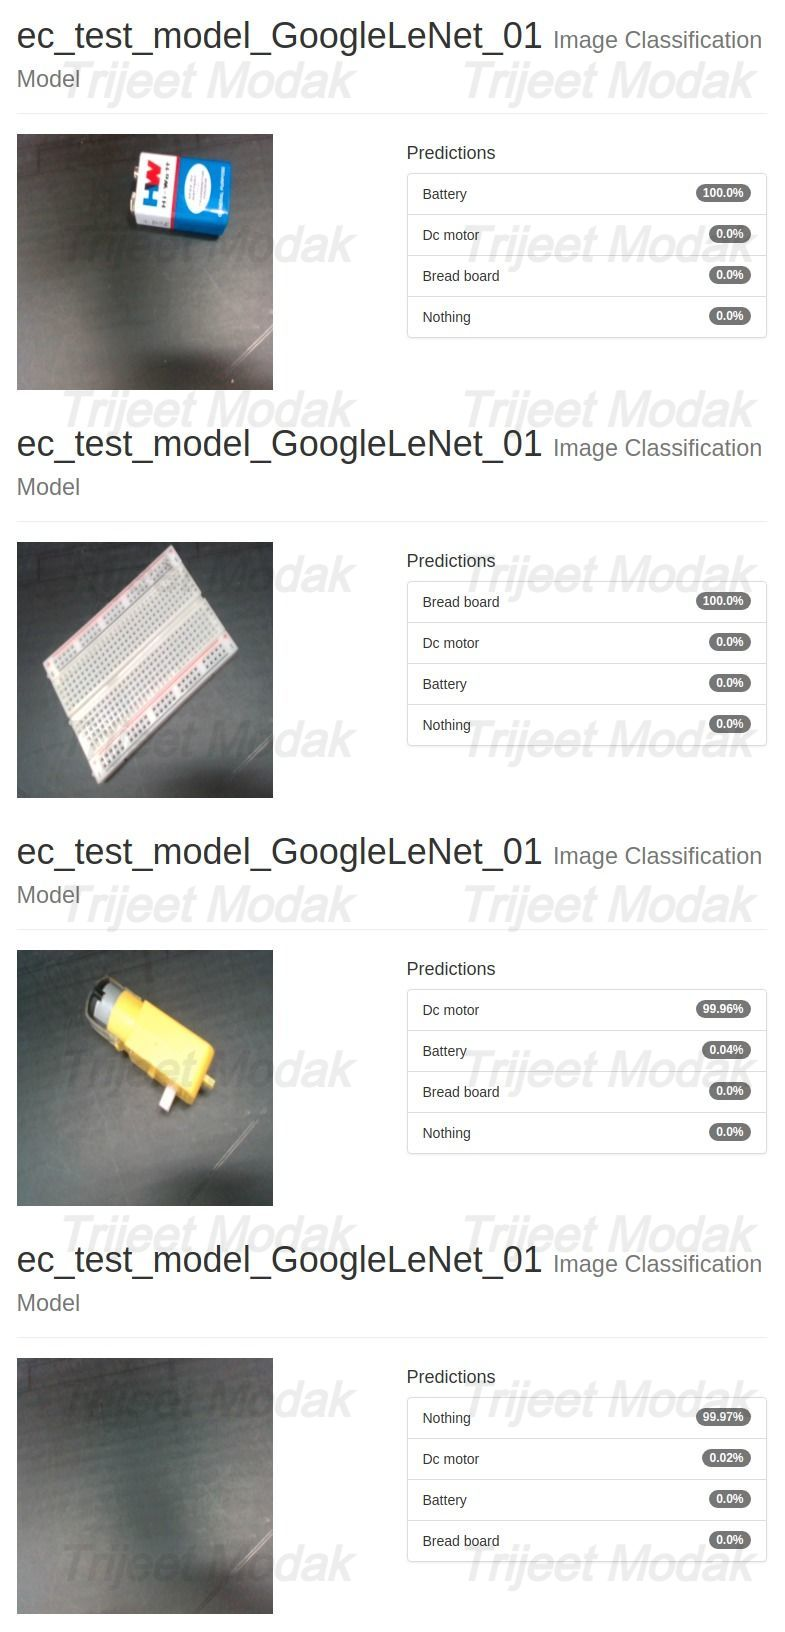
\includegraphics[scale=0.325]{imgs/detections.jpg}
    \centering
    \caption{Model 2 loss/accuracy vs epoch curve}
    \label{fig:detections}
\end{figure}

\section{Discussion}
It is quite astonishing that GoogLeNet was able to train itself using only about 100 images per class for the second model with over 95\% accuracy. One reason for this could be because there were only 4 classes to predict from and there were no subclasses in the dataset. 

Although a high accuracy is always desirable, it is important that it doesn't take too long to make an inference especially in a realtime scenario. GoogLeNet seems to be fast enough to be used in real-time object recognition operations for robotic inference projects. 

\section{Conclusion / Future work}
GoogLeNet was used to model two different scenarios of object classification/recognition, one with a set of supplied data from a conveyor belt and another set that was manually collected while doing the project. In both cases GoogLeNet was able to predict the correct class of the object almost always with a very high confidence value. The results were promising and met the project requirements.

\bibliography{bib}
\bibliographystyle{ieeetr}

\end{document}